\chapter{Session 1}
\section{Preparation}
The characters will start in their HQ, asleep. Little do they know that they're in the process of being robbed. Luckily, these aren't the most intelligent thieves. They accidentally bump into all sorts of things, such as cleverly hidden warding glyphs.

'First journal of Barakas Taruth'. Ondervraagde heet Ned stablemaster. Henk is boven.

\section{Report}
Characters were a bit too confident, and were ambushed by the lurkers. This caused some immediate trouble with line of sight / confined space. Overall, went well; damage output is pretty high.

Next session, they'll start with a post-combat discussion involving Arbelly, after which it is sleep and hitting the road.

\chapter{Session 2}
\section{Preparation}
Tested d20. Need to make some brushed combat maps, and sprites. This sessions characters will discuss the journal with Arbelly. Arbelly also mentions rumours of a strange coated-cat living around there, whose pelt he'd love to go after. Alas, it is a three-day trip and he has to watch the fort. After that, they should move to the ruins. During the trip, they will be ambushed by some wildlife at night (woken by their guard or by an attack). Afterwards, as they close in on the ruins they will encounter a scouting party that is looking for the back entrance. Traps have been lied down, but they're quite easily spotted. Can be used in combat. The scouts have been sent out because of the front-end sentinal, noted in the journal.

The back-entrance has become the liar of a cougar, strangely patterned because of the effects of the magic seal \href{http://www.dandwiki.com/wiki/Wild_Cats_(4e_Creature)}{[stats]}. As the party enters the liar, it jumps them.

It is extremely unlikely that they make it this far in one session. The next session picks up where they left it, or starts with the puzzle.

\section{report}
The characters have not even reached the first combat planned out, and have ended during the night. They did spend a lot of time roleplaying. I'm not sure about the content.

\chapter{Session 3}
\section{Preparation}
\begin{itemize}
\item Handwritten notes for the Journal (Translated by Arbelly).
\item Cougar Print
\item Battlefield: Camp at night.
\item Battlefield: Running into scouts
\item Battlefield: The back entrance.
\item Sprite: Human Goon
\item Sprite: Halfling Thief
\item Sprite: Cougar
\item Sprite: Gray Wolf
\end{itemize}

Encounter at night (easy, 375xp):
\begin{itemize}
\item 3 Gray Wolves, Lvl 2 Skirmisher, MM (125xp)
\end{itemize}

\section{Report}
Starting immediately with the encounter at night, the party quickly immobilizes, burns and annihilates whatever it is that attacks them. The tent of Maghir, however, is destroyed by his hammer and the central pole incininerated by Ilyena. However, after combat it is restored using artificer magic.

\section{preparation}
Encounter the scouts (easy, 850xp incl. traps):
\begin{itemize}
\item 2 Halfling Thief, Lvl 2 Skirmisher (125XP), MV
\item 4 Human Bandit, Lvl 2 Skirmisher (125 XP), MV
\item 1 False-Floor Pit, Lvl 1 Warder Trap (100xp), DMG
\end{itemize}
\section{Report}
During the watch, they heard the snarling of a cougar. When they turned to investigate, they found the pit trap and circumvented it. They found one human bandit with a ripped out throat. They used several kinds of magical healing, including paladin powers, and the man might survive. (1 throw failed).

The accidentally hard encounter (Human goons to bandits) was successfully managed by the party. While the dwarf took a beating, the other two controlled and demolished the entire company. They took one prisoner using a Daily Sleep spell. 

\chapter{Session 4}
\section{Preparation}
LVL 3 treasure parcels. 

Encounter the Scots: Lvl 4 magic item (bag of holding), 3 potions of healing, 2x 100gp jewellery, 80 gp. (parcels 3/5)

\section{Report}
The party spent the entire session trying to get information from the prisoners ( near-death bandit, sleeping bandit). They got a bit of information; Kairon, the concorde, the back-entrance (and finally, Ilyena revealed her knowledge), Giovanni (boss, father Kairon, both thieflings), maybe more. Also, some excellent advise for getting kicked in between your legs.


\chapter{Session 5}
Encounter the Beast (hard, 750):
\begin{itemize}
\item Leopard, Lvl 3 Solo Lurker (750xp),\href{http://www.dandwiki.com/wiki/Wild_Cats_(4e_Creature)}{[internet]}
\end{itemize}
\section{Report}
The party spend some time exploring before finally entering the cave, where they were promptly ambushed by the magical cougar. It did some heavy damage but was ultimately defeated.


\chapter{Session 6+7+8}
\section{preparation}
Cougar fight assigned: lvl 7 magic item, stalwart belt, 1potion of healing, 100gp gem, 75 gp. (parcels 1/7)

Cougar Quest reward: 600 gp (parcels 6/8)

Magical backdoor puzzle. You enter a large room. In the centre is a spherical pattern; when you walk closer, it lights up in arcane blue, revealing a pentagram. On the other side of it, you see a great door with a magic seal on it (shimmering energy field). The alcoves light up in order, so that the party is very much railroaded.

In the alcove on your left, two demon statues stand. One has an orb in hand, the other doesn't. As you move closer, a sound is heard from the orb-less statue. "Give me the orb of power!", it says. The trick is to take the orb from the other statue, but not to give it to the statue. Power isn't given. If you fail to keep it, 3 imps (monster vault, lvl 3 lurker, total 450xp) are summoned invisibly and attack the party.Otherwise, the imps are summoned in the circle. In the first case, the imps screech "Power is never freely given!". In the second case, they screech "power must be taken" while they are summoned. It should be abundantly clear that the orb is power. In fact, it is a magical item that will help the party. The `orb' is a polished dragon-shard, something that will call out to Maji (due to artificer) and to Theodore (due to interest). (Parcel 8/10).

To the right and behind the point of entry, a second alcove stands. Here, a statue sits with two orbs. As you approach, the statue turns its head. A voice rings out. "The final words; you hold power. Now answer me true; what do you know?". Any answer that is not equal to "nothing" is false; however, the party does not notice. Either way, the response will be "Thou have spoken fairly. Continue on the way to power".

The final alcove holds a statue of a succubus. However, as you approach the activated alcove, you see no succubus. Instead, a slender woman of graceful curves sit there. She looks at the party, especially Maji, with big, teary eyes. "Help me!", she asks imploringly, " the priests chained me up and left me here, enchanted. I have not seen my parents since they took me here". She cries a bit.

Look, obviously it is a chained up succubus. The verse is inverted, and she tries guile to get free. When she is free, she reveals her form and keeps free by her power. The party can try to get opportunity attacks in, but whenever they attempt so the armour shimmers. It's magical armour, of course (Parcel 5+6). There's a catch - it is, most definitely, female succubus armour. Ilyena can choose to wear it, and it fits her well. Otherwise they can sell it. Either way, it sounds amusing to me. The succubus will call out its magical properties in the fight. 

After the succubus fight, the door opens. Succubus armour, Shimmering Armor +2 (AV p51).

Personal affections (jewels, treasured toys) can greatly affect a succubus formed from a deranged virgin maiden.

\section{Succubus Encounter}
HP is 160. Defences are 5 lower. The succubus cannot fly until bloodied. It has resistance to fire. Melee attack 1d10+6, +9 vs AC. Charming kiss, melee 1, +9 vs Will. Target has a -2 versus the succubus. Lasts until an ally hits it, the succubus dies or the succubus kisses someone else. Dominate, ranged 5, +8 vs will. Dominate target until next turn. Keep the change shape. Loyal consort; share half damage with kissed target. The succubus has magical armour that prevents opportunity attacks.

\section{Report}
De succubus has been defeated. The girl/woman, Jewel, was once turned into a succubus by a combination of being trapped and a demonic artifact. Turning a virgin maiden into a succubus this way might be reverted, according to a bit of profound lore remembered by Theodore. Once, a wizard used a bit of woman's blood, freely given, to bind a succubus to him as an arcane familiar, then slowly influencing it to reduce the influence.

After the encounter and the ritual of binding, the party turns to the door. Slowly, the magic - which was being drained from the succubus trap - has seeped away, so that the door is now free. At the top of the door, Abyssal glyphs read (according to Jewels): "A great wizard has big/magic hands". Theodore knocks using mage hand and the door asks: "Who is it?". A bit of banter ensues. Finally, they notice the lever in its mouth and use mage hand to open the doors.

Three poker-playing guards look befuddled, then run. Grasping shadows knock them to the floor, unconscious. After dragging them away, binding and reviving them, the interrogation starts. Whois your boss? Henk. Who is his boss? Shannon. Who is her boss/ Richold. Who is his boss? Captain Calis. Who is the big boss? Giovanni. Is Kairon here? Yes. Maybe you should ask Dirk, the one with the bleeding wound. The party makes a deal with the goons: For a bottle of vodka, they will ignore the party passing through. It's their house, after all.

\chapter{Session 9}
\section{Preparation}
\begin{itemize}
\item parcel 1: Shimmering armour +2 (Ilyena)
\item parcel 3: lvl 6 item, hammer (Session 10)
\item parcel 5+6: 670 gp + art object, final loot
\item parcel 7: 100gp + 2 pots
\item parcel 8: 1250 gp art
\item parcel 9: 90gp + pot
\end{itemize}

Solo Common Bandit, Henk's brother Zarrik. HP is 160 Hp. Defences: AC 18, Fortitude 12, Reflex 16, Will 14, 2 action points, extra standard action.

As the party enters the tunnel, they note that the floor has a pattern on it. It doesn't actually do anything but it is fun to point at. Later, they see the pattern change and a dead bandit lies on the floor. As they approach, they note (Perception DC 15) a character standing in the shadows/gloom. Approaching the dead bandit, who they see has a large gash across his shoulder, triggers a double-trap: \href{https://www.dandwiki.com/wiki/One-way_barrier_(4e_Trap)}{a barrier} with two \href{https://www.dandwiki.com/wiki/Scything_Blade_Trap_(4e_Trap)}{A rusty scything blade}. The triggering squares are the three in front of the bandit. At the same time, the character in the shadows steps forward.

Zarrik stands there, Sword drawn. Zarrik is a small human wearing a golden chain. His leather vest is open at the front, showing an abundance of breast hair. On his back, he carries a large, polished crossbow. He carries a longsword with visible decoration around its pommel and crossguard. The scabbard is red leather with golden fringes. He has a large belt with all sorts of pouches and daggers - about 20 cm high. 

Zarrik doesn't engage, nor talk - he just stands there, arms crossed. A perceptive character sees that this means both hands are near throwing daggers. As you move on, you will either activate the trap or he will (using the daggers). His whole purpose is that you disable the trap so that he has a way out. If you engage him, you can kill him for bonus loot. If you don't, he will set up in HQ town so that you have a link to the black market etc. His story is that his brother - whom he hadn't seen in almost ten years, since he left for the larger cities when reaching majority - asked him on  as a mercenary, and that he had little else to do as he was coming to visit his family. He now realises his brother is in over his head - in fact, that's the dead man lying there - and he wants out. 

Occupation: A shady back-alleyway character that has dealings with everything shady. Values honesty and what he considers good deeds over the law. His motivation is a combination of greed and trying to protect the poorer people from praying factions such as the copper Concorde. Usually stands with arms crossed. He is engaging in a rough way, often giving in to booming laughter. Slightly condescending in the you-did-not-grow-up-on-the-street way. As a talented and well practised rogue, Zarrik can give the players a map detailing traps lied by the Concorde around the compound - which is valuable just for being a map. Zarrik often talks to his sword, which he calls Maria. If you wonder where he got it, he says he got it outside of a shop that was there one day, then gone the next day. It was in the trash, for some reason he doesn't understand.

Report (bullet points)
\begin{itemize}
\item Golden Tankard; Pub where Theodore saw Zarrik
\item The dead guy isn't his brother
\item They paid Zarrik for the map with fool's gold
\item They got a red/black key from the main chamber. What is it?
\end{itemize}

\chapter{Session 10}
After the interesting encounter with Zarrik, the characters move on. Having bought - for fool's gold - the map of the dungeon Zarrik made (fig~\ref{fig:firsttemple}), they confidently step into the dungeon.
\begin{figure}[h]
    \centering
    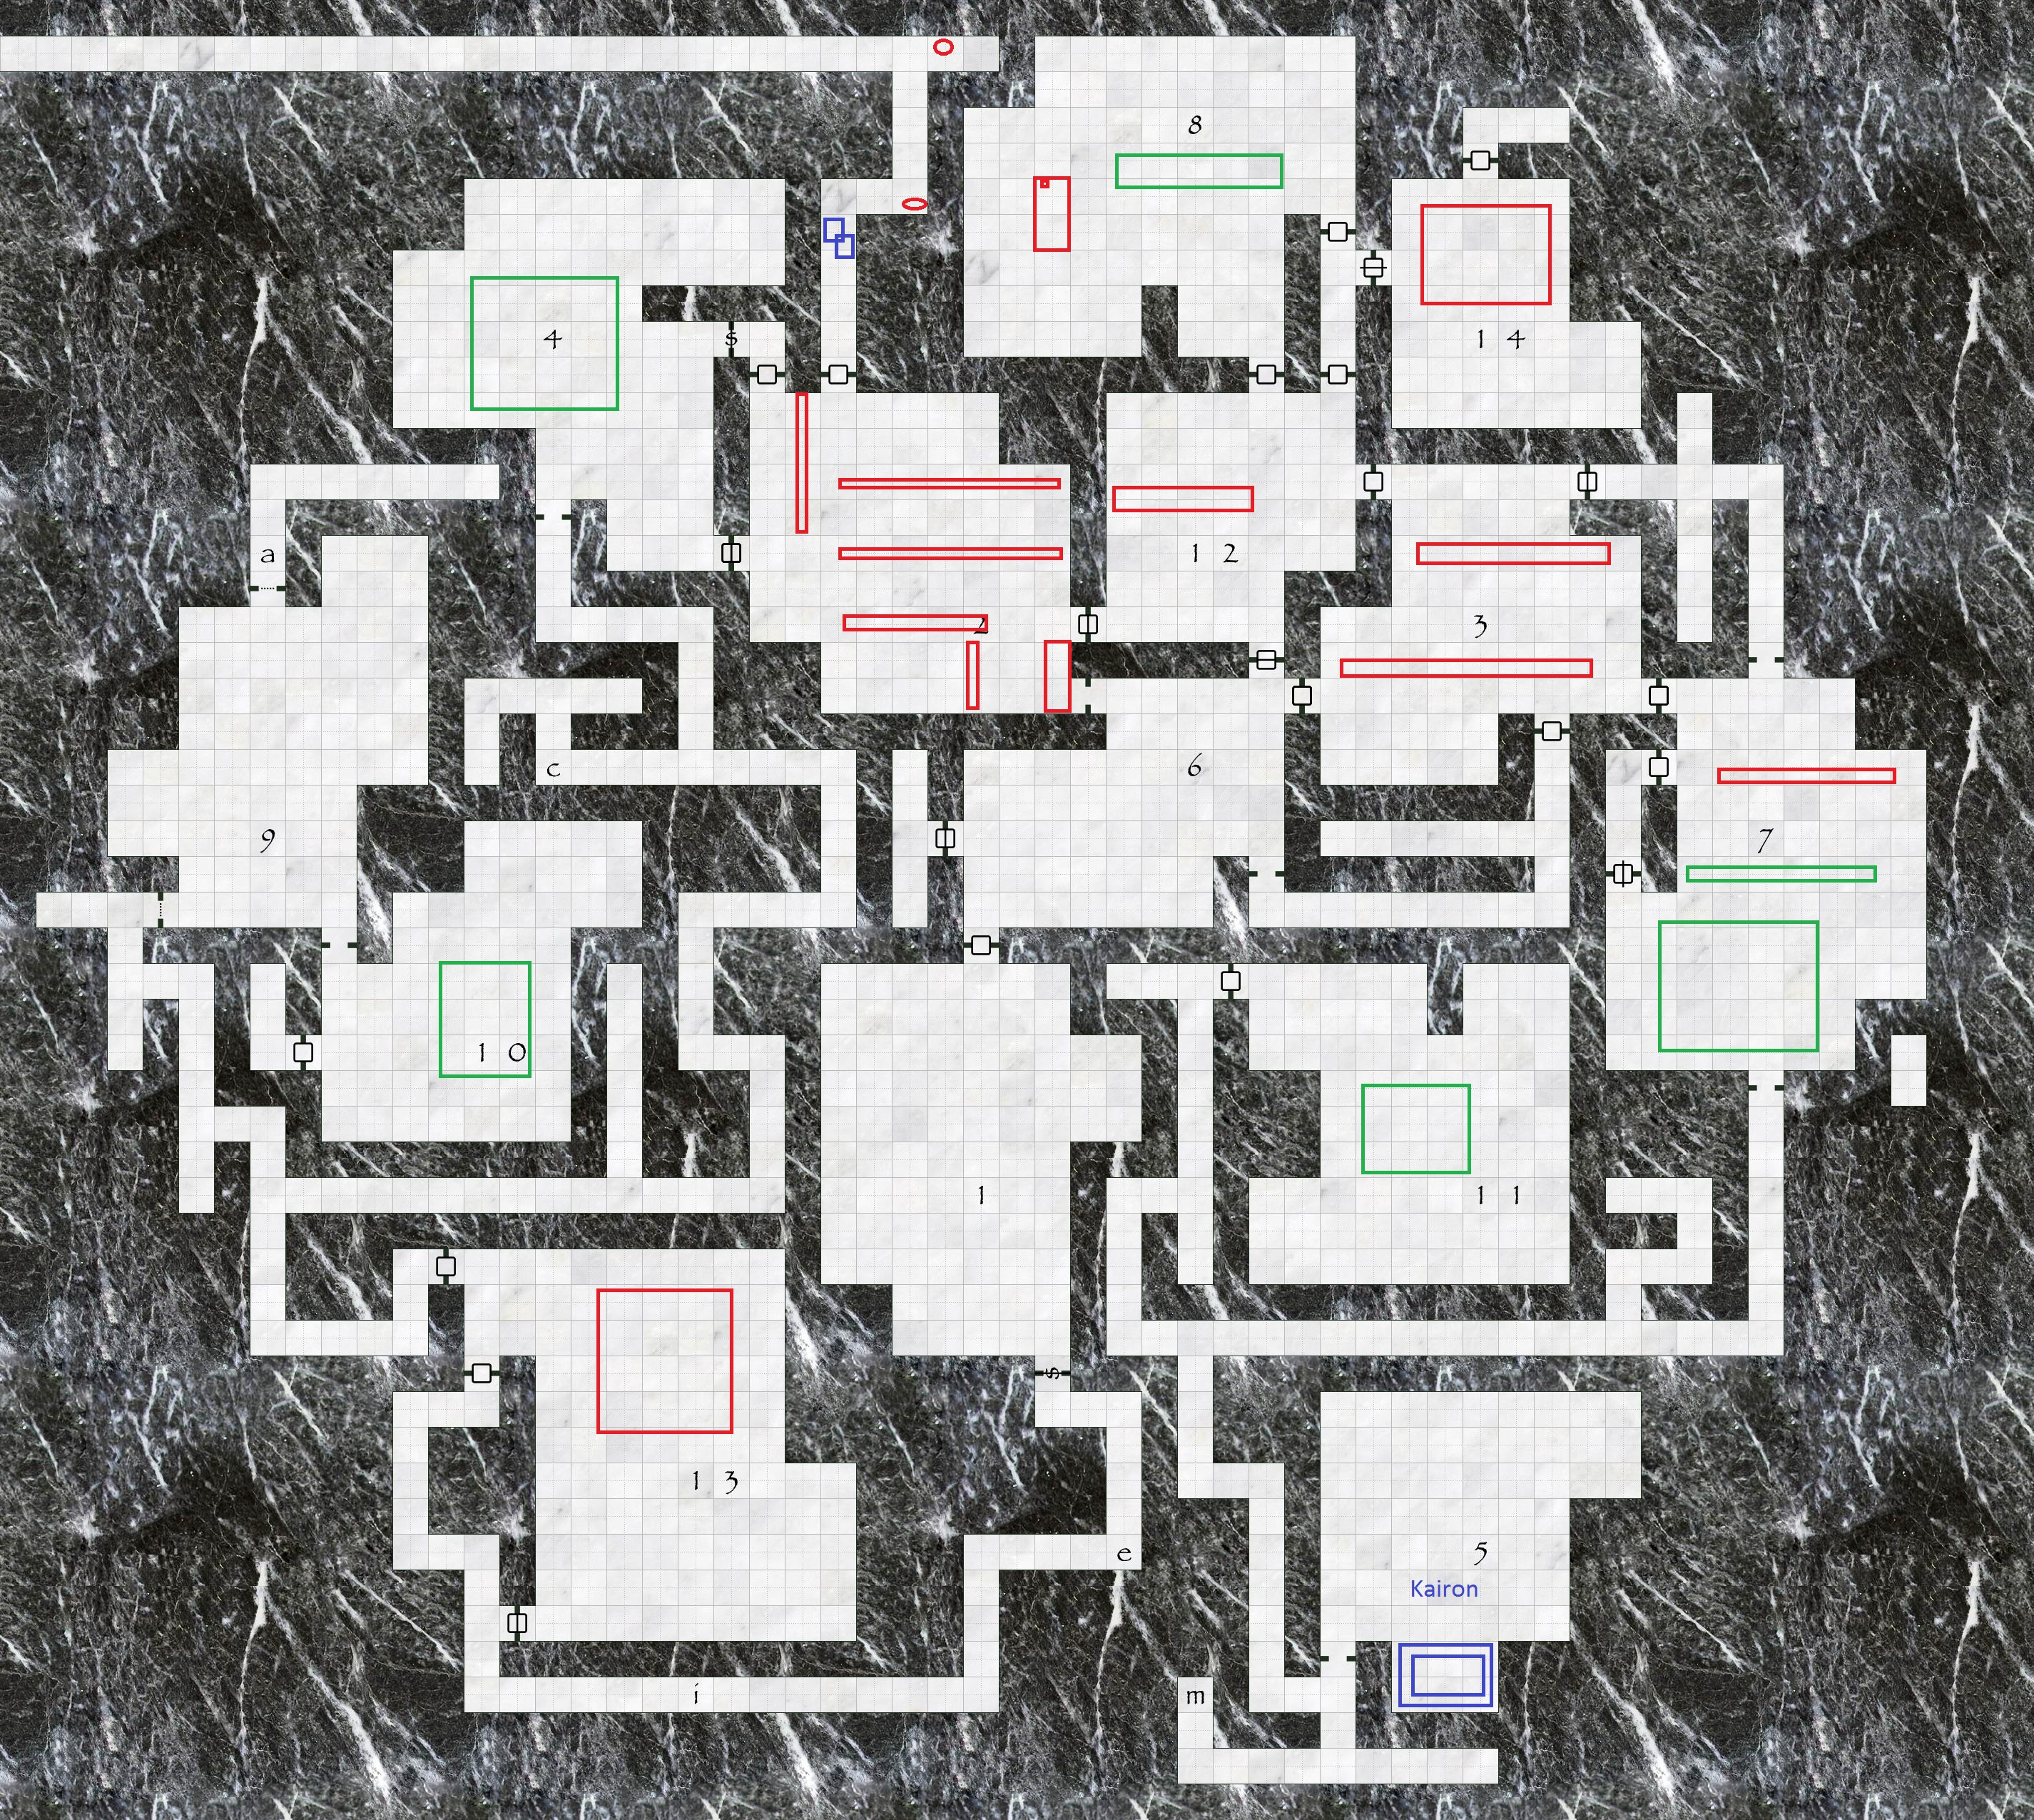
\includegraphics[height=.5\textheight]{fig/firsttemple.jpg}
    \caption{\label{fig:firsttemple} Map made by Zarrik.}
\end{figure}

The first thing they notice, however, is a floor littered with frozen bodies. While the floor is charred, they can quickly note fire traps have been frozen by something. On the middle of the room, light shines down - part of the ceiling collapsed. On closer inspection (DC 20) they note that it didn't come down naturally - it looks too clean, lasercut. Into a convenient liar for a white dragon - a young white dragon lands, roaring! (Monster Vault, Young White Dragon, Level 3 Solo Brute, XP 750).

Report:
\begin{itemize}
\item De oorlog van 1924 draken vs dwergen, iets met een opgegeten mount/geit met zadel + persoon
\item traps! traps!
\item Draak sluit af met 'Verborgen Kennis? Wat heb je daarvoor over' en vliegt weer omhoog.
\item Ilyena vind het verloren boek: Demonotelicom, Levels of Demonology
\item Manji vind: De weg van de Dwerg
\item Theodore vind: De Tao, wiens titel lichtblauw oplicht
\item Secret way into vault 9
\end{itemize}


\chapter{Session 11}
Preperation:
\begin{itemize}
\item Preparation: Goblin Hex Hurler as Human Wizard, 2 Dwarf Clan Guard, 4 Dwarf Warriors
\item Gnoll HuntMaster, 2 Deathpledged Gnoll 
\item Kissing Maiden, DMG 2 p66
\item Caustic Geyser as Fire Geyser, DMG p91, DC 19 for all checks, +8 vs reflex, 2d8 acidic damage
\end{itemize}
Report:
\begin{itemize}
\item Vault 9 contains sacrificial hammer now (Parcel 3)
\item Plus art item from figure~\ref{fig:emperor}. (Parcel 8) Added value of 1000 gold because I forgot looting creatures
\item Loot: 100 gold, 2 healing potions, 4 chainmail, 2 platemail, 6 warhammers, 1 heavy shield, 80 crossbow bolts, 4 crossbows, 8 throwing hammers, leather robes, staff, spellbook (vexing cloud, stinging hex, blinding hex), 3 leather armours, 2 light shields, 2 longspears, 1 handaxe, longbow, 30 arrows
\end{itemize}

\begin{figure}[hb]
    \centering
    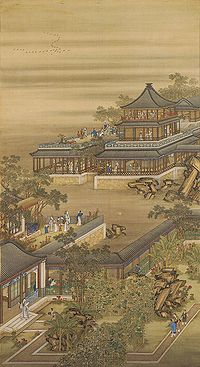
\includegraphics{fig/Portraits_of_the_Yongzheng_Emperor_Enjoying_Himself_during_the_8th_lunar_month.jpg}
    \caption{\label{fig:emperor} Portait of the Yongzheng Emperor Enjoying Himself During the 8th lunar month, by (fictional) Kong Le'Mao-Tze}
\end{figure}

Een vrouwelijke dwarf clan guard wordt vrijgelaten, en is er van overtuigd dat de party ook Concorde is. Ze vlucht de dungeon uit en wordt ergens kapper (haar andere droom).

De party loopt kamer 10 in, die gekoeld is en waar een massieve stenen deur met een magisch symbool enigsinds teveel magie afgeeft. Ze besluiten hier niet te proberen de deur over te forceren. Aan de andere kant is een kast en een magisch tapijt. De kast bevat boeken over elementals, maar dit is niet zo interessant. Wel heeft Theodore de ingeving om het tapijt mee te nemen.

In de gang tussen 10-13 bevechten onze heldene en rust-monster momma (brute) en haar kinderen (swarm). Deze hadden net 2 dwarven clan guards vermoord/verminkt en hun items opgegeten. Vervolgens is er een obstructie, waardoor de rust monsters opgesloten zaten. Jewel heeft een rust monster egg in Manji's bagage/persoon verstopt. Heh.

Kamer 13 heeft een water-filling chamber, met een standbeeld van de serpent-maiden cult binnen het oude thieflin rijk. De kamer bevat veel kasten e.d., welke genoteerd staan op de kaart.